\documentclass[10pt]{article}
\usepackage[margin=0.72in]{geometry}
\usepackage{amsmath,amssymb,graphicx,booktabs,xcolor,hyperref}
\definecolor{ink}{HTML}{253C59}
\hypersetup{colorlinks=true,urlcolor=ink,linkcolor=ink}
\setlength{\parindent}{0pt}\setlength{\parskip}{6pt}
\begin{document}
{\Large\bfseries\color{ink} Compact coset spectra for Curve25519}\par
{\small 23 November 2026 \quad Proposed representation; solver operation still open}

\textbf{Purpose.} Replace an explicit product over $k$ cosets by six unknown
coset labels, while retaining the five unknown section coefficients and every
original lifting condition. This report derives the written contract and
identifies the exact missing solver object. It contains no new timing,
coefficient-discovery result or exponent estimate. Producer standing is unsigned.

\textbf{Candidate algebra.} Under the fixed original positive-window,
exact-order and field hypotheses, retain the monic sextic $S(c)$ and put
\[
 A_S=\mathbb F_p[X]/S,\qquad
 g=T_q\!\left(\frac{A}{2X+A}\right)^2,\qquad
 b_j=\operatorname{Re}((h^q)^j)^2.
\]
The old map guard makes the denominator invertible. The proposed membership
equations are
\[
 \delta\operatorname{Disc}(S)=1,\qquad 1\le j_i\le k,\qquad
 \det(TI-M_g)=\prod_{i=1}^{6}(T-b_{j_i}).
\]
Here $M_g$ is multiplication by $g$ on $A_S$. The labels are unknown;
repeated coset labels are allowed. Keep the existing rational torsion guard,
target charts, $Q=[8]R$, and original sign/raw-index/group replay.

\textbf{Written equivalence.} Write $H(T)=\prod_{j=1}^{k}(T-b_j)$.
Original membership implies $S$ is squarefree and $H(g)=0$, hence the
displayed spectrum by the classical eigenvalue theorem. Conversely the
spectrum gives $\chi_g\mid H^6$. Cayley--Hamilton yields $H(g)^6=0$;
the discriminant guard makes $A_S$ reduced, hence $H(g)=0$. Clearing the
invertible map denominator recovers the old membership remainder. This
argument assumes coefficients in $\mathbb F_p$ and the preceding norm/lifting
contracts; its full native and Lean binding remains open.

\textbf{Guard control.} In $\mathbb F_{101}[X]/X^2$, multiplication by $X$
has matrix $N=\left(\begin{smallmatrix}0&1\\0&0\end{smallmatrix}\right)$.
Its characteristic polynomial is $T^2$ and $N^2=0$, but $N\ne0$.
Thus matching a repeated spectrum does not imply $H(N)=0$ for $H(T)=T$.
The finite Lean target checks exactly these three matrix identities; it
does not certify the full section compiler or an actual malformed section.

\textbf{Representation budget.} At fixed arity, binary Chebyshev and binary
unknown-index chains give a written $O(\log q+\log k)$ arithmetic-circuit
construction, with guards and coefficient-bit work retained. At $k=20633$,
six index words and six range-slack words require 180 Boolean inputs before
optional sorting. No such native circuit was built in this assessment.

\textbf{Required comparator.} The existing original point circuit already
has polylogarithmic index chains (1059 variables /1089 quadratic equations
on its frozen six-point fixture, inherited unsigned evidence). Reducing the
expanded 4.6-million-wire section program alone would not establish a new
scaling advantage. Both representations must receive identical public targets.

\newpage
{\large\bfseries\color{ink} The solver dimension is the missing quantity}
\begin{center}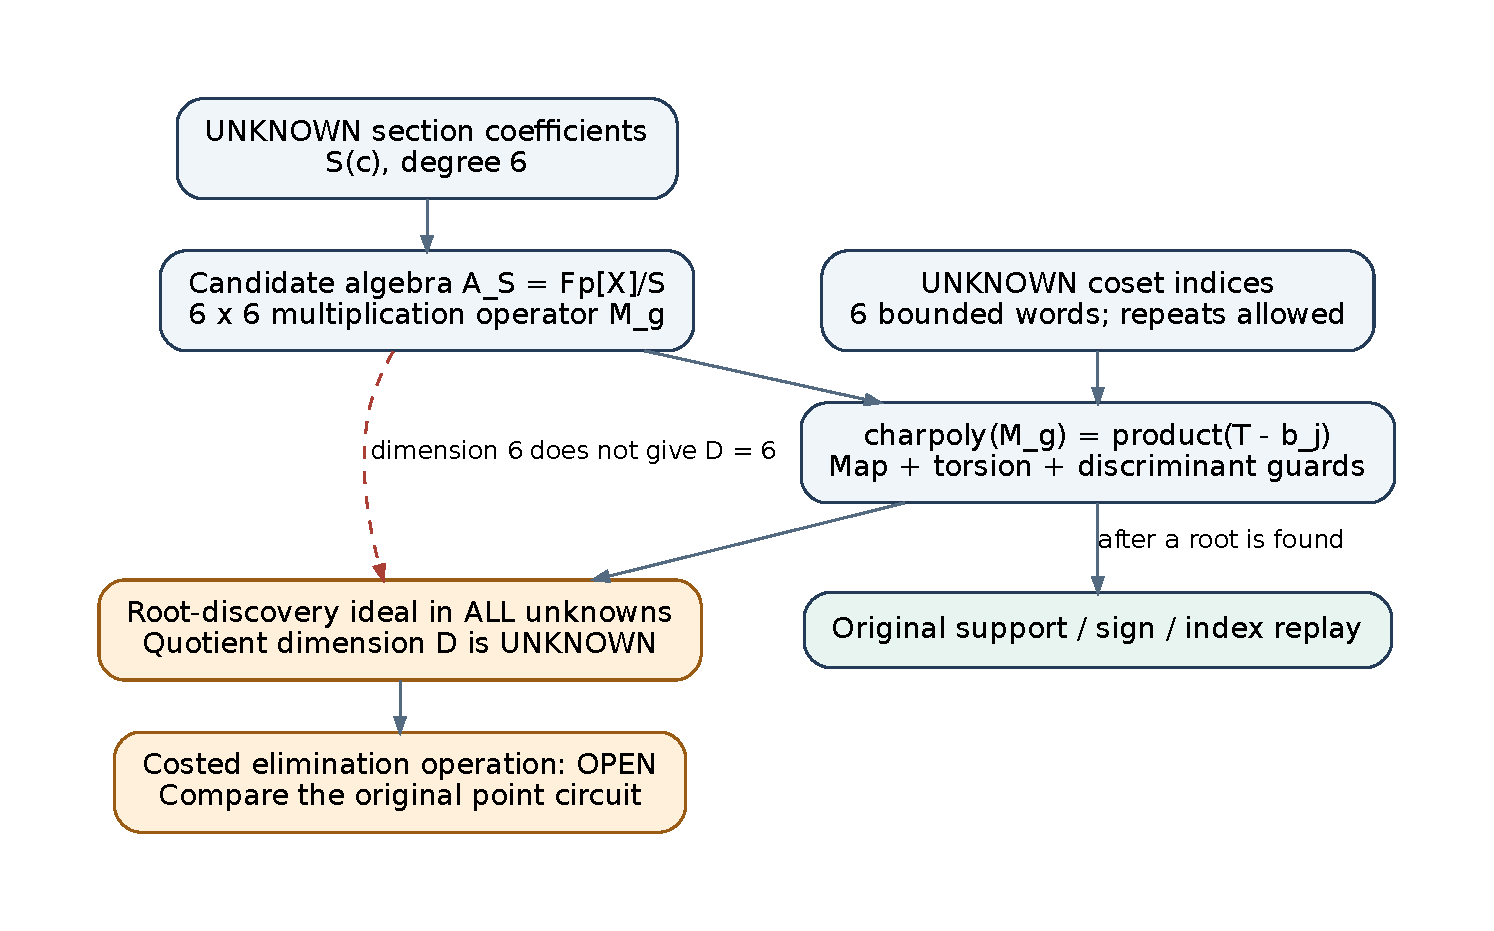
\includegraphics[width=0.90\linewidth,height=3.55in,keepaspectratio]{diagram.pdf}\end{center}
\vspace{-6pt}
\textbf{Two different algebras.} $A_S$ has dimension six after choosing a
coefficient tuple. A root solver faces the ideal $I$ in all coefficient,
index-bit and guard variables. If it is zero-dimensional, the relevant
dimension is
\[D=\dim(\mathbb F_p[c,\text{bits},\text{guards}]/I).\]
Neither this property nor a bound on $D$ follows from $\dim A_S=6$.
Sparse FGLM requires the solution-ideal basis/multiplication matrices, with
construction cost, degree and sparsity accounted. Substituting $D=6$ from
the candidate algebra is an invalid use of that algorithm.

\textbf{Explicit phase gate.} If the effective base has size
$B=\ell^b$, complete cold query work is $B^{\gamma+o(1)}$ and inverse useful
yield is $\ell^{y+o(1)}$, collecting $B$ useful rows costs exponent
$b(1+\gamma)+y$. At the conditional six-sum model point $b=1/6,y=0$, this
phase requires $\gamma<2$ for strict exponent below $1/2$. Rank, setup,
kernel, recovery, field filtering and memory remain separate obligations.

\textbf{Decision and next test.} Keep the guarded spectral contract as a
candidate; reject the constant-dimensional-FGLM inference. Before another
solver run, specify a concrete elimination operation that avoids all-index
branching and unpriced solution-matrix setup. Then qualify public-only
unknown-coefficient discovery, original replay and the matched point-system
comparator on a declared blinded finite domain. Caps and incomplete output
are not absence certificates. No campaign is scheduled by this report.

{\footnotesize\textbf{Sources.}
\href{https://arxiv.org/html/2007.12573v2}{Cox, eigenvalue theorem, \S1};
\href{https://arxiv.org/pdf/1304.1238}{Faugere--Mou, Sparse FGLM, \S1.2--2.1};
\href{https://doi.org/10.1007/978-3-642-55220-5_3}{Faugere et al., EUROCRYPT2014, \S3.3}.
Full retrieval scope/gaps and internal source pins: SOURCES.md and PROOF\_MAP.md.
Symmetric variables and matrix methods are classical; no novelty clearance
is claimed. Companion REVIEW.md carries the complete written argument.}
\end{document}
